
\section{Dataset Description}
\label{sec:datasets}


 
The author team coordinated the release of four public, AI-ready datasets, each derived from a neutrino detector capable of searching for NLDBD. Each data point corresponds to a physics \textbf{event} recorded by the respective detector; we therefore use the terms event'' and data point'' interchangeably throughout this paper. Because these detectors rely on different detection technologies, their event span substantially different modalities. Our central benchmarking task is to distinguish signal-like events from background-like events based on event topology, even though the topology manifests differently across data modalities. 

As shown in Figure~\ref{fig:signal_background}, the relevant topological signatures appear differently across detectors and data modalities. The \textsc{Majorana Demonstrator}~\cite{Arnquist23} is a high-purity germanium detector experiment. Event in the \textbf{MJD} dataset can be represented as 1D waveforms with 3,800 time samples. Event topologoy information is primarily encoded in the waveform's rising edge: signal-like events tend to exhibit a clean, single-step rise, whereas background-like events more often contain multi-step structure. NEXT~\cite{Novella23} is a gaseous-xenon time projection chamber (TPC) experiment. Event in the \textbf{NEXT} dataset~\cite{next_ml_dataset} can be represented as sparse 3D point clouds, where each point represents a localized energy deposition. Here, topology is encoded geometrically: signal-like events typically form a continuous track with high-energy clusters at both ends, while background-like events more often exhibit only one such cluster. The SuperNEMO~\cite{Petro25} experiment is a tracker-calorimeter experiment. Each event in the \textbf{SuperNEMO} dataset~\cite{supernemo_ml_dataset} can be represented as a similar point-cloud structure compare to NEXT, but the points tends to align more in a straight line~(track). Signal-like events will tend to have two tracks starting from the same position, while background-like events tend to exhibit a gap between the two tracks. Finally, EXO-200~\cite{Anton19} is a liquid-xenon TPC experiment. Each event in the \textbf{EXO} dataset can be represented as a sparse 2D images, in which event topology appears as localized "bump" strucuture. Signal-like events tend to have only one such bump, while background-like events tend to have multiple bumps.

% The collaboration requests that analyses built on this release also cite the original EXO-200 result obtained with the complete dataset~\citep{exo200_prl2019}.

% ----------------------------------------------------------------------------
% Figure: one representative image per experiment.
%
% NOTE(Vivek): the four images below are placeholders generated locally
% (labeled boxes, not real photos) because this environment cannot fetch
% or download binary image files from the web. Suggested real replacements,
% each with a usable credit line, are listed in the chat reply alongside
% this file -- swap them into figures/ under the same four filenames and
% this block does not need to change.
% ----------------------------------------------------------------------------
\begin{figure}[t]
    \centering
    % --- Row 1: Signal ---
    \textbf{\small Signal}\par\smallskip
    \begin{minipage}[b]{0.23\linewidth}
        \centering
        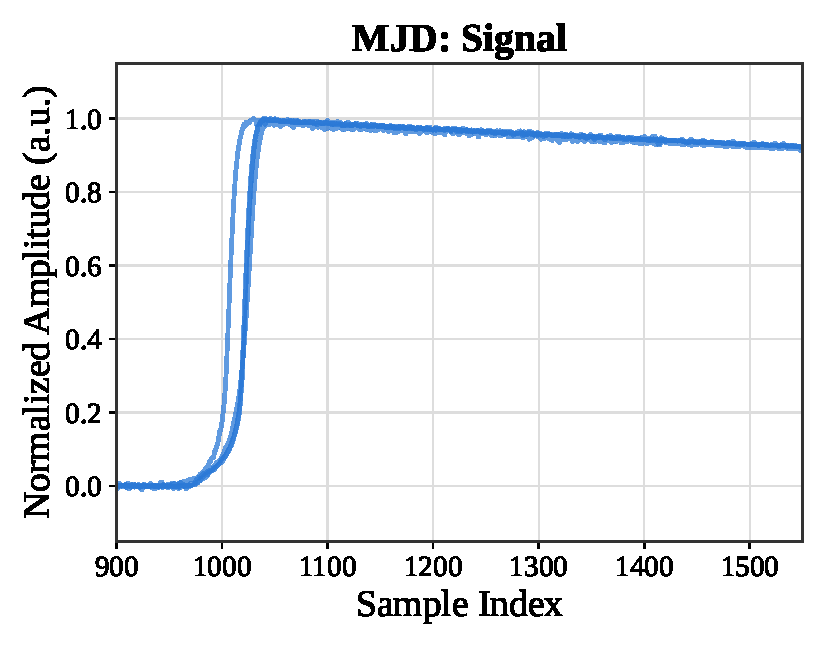
\includegraphics[width=\linewidth,height=3.4cm,keepaspectratio]{dataset_description/Images/mjd_signal.pdf}\\[2pt]
        {\small (a) Majorana Demonstrator}
    \end{minipage}
    \hspace{2mm}
    \begin{minipage}[b]{0.23\linewidth}
        \centering
        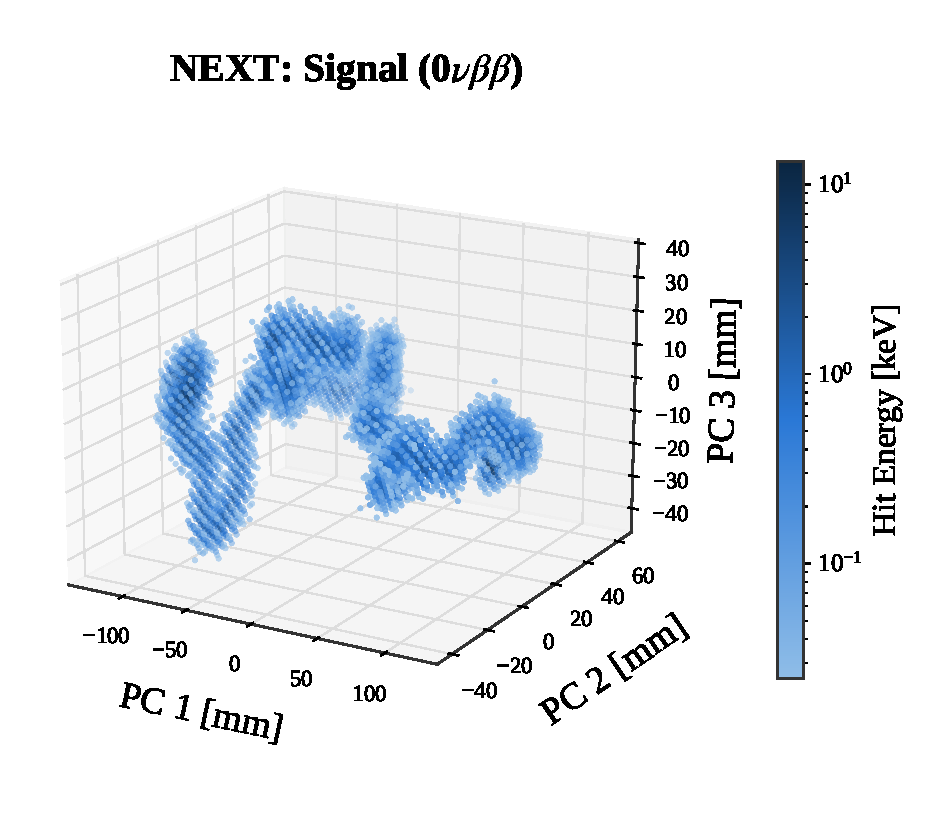
\includegraphics[width=\linewidth,height=3.4cm,keepaspectratio]{dataset_description/Images/next_signal.pdf}\\[2pt]
        {\small (b) NEXT}
    \end{minipage}
    \hspace{2mm}
    \begin{minipage}[b]{0.23\linewidth}
        \centering
        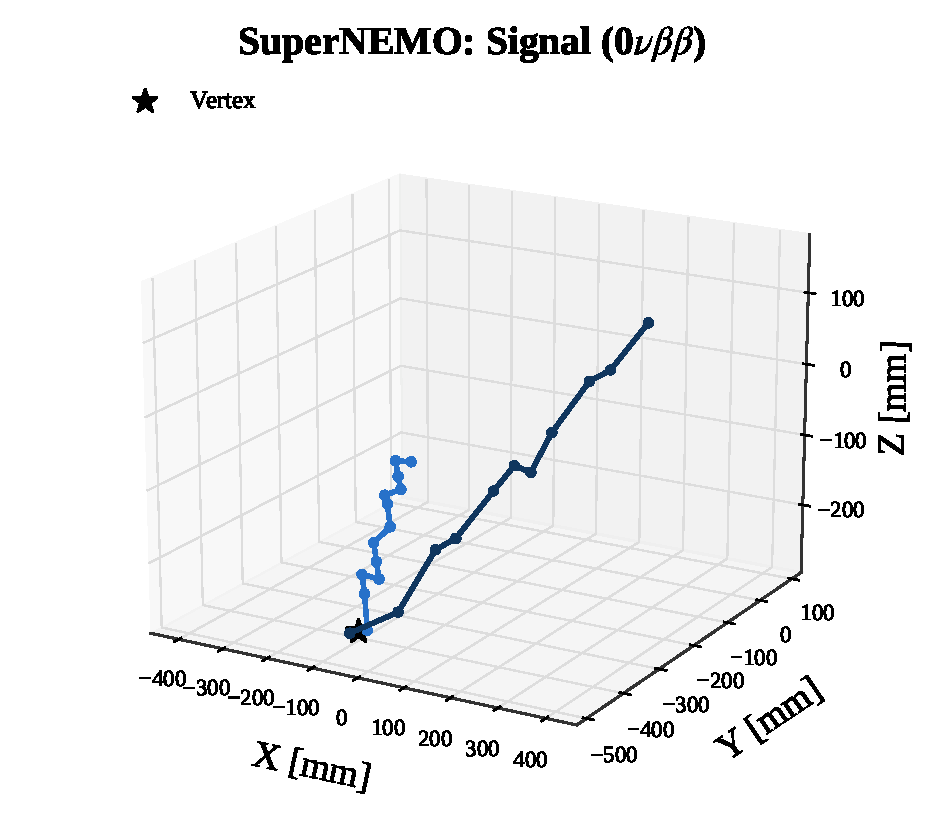
\includegraphics[width=\linewidth,height=3.4cm,keepaspectratio]{dataset_description/Images/supernemo_signal.pdf}\\[2pt]
        {\small (c) SuperNEMO}
    \end{minipage}
    \hspace{2mm}
    \begin{minipage}[b]{0.23\linewidth}
        \centering
        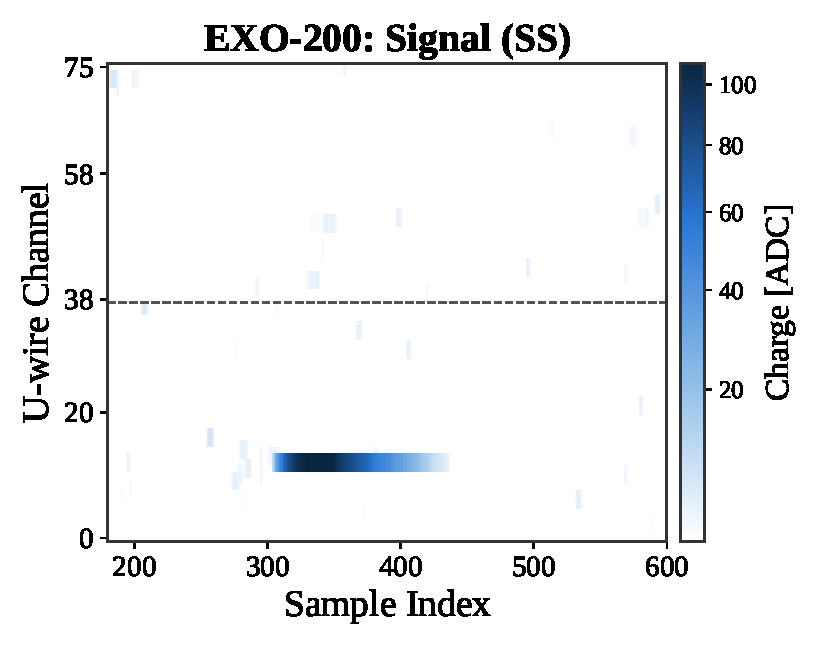
\includegraphics[width=\linewidth,height=3.4cm,keepaspectratio]{dataset_description/Images/exo_signal.pdf}\\[2pt]
        {\small (d) EXO-200}
    \end{minipage}

    \vspace{4mm}

    % --- Row 2: Background ---
    \textbf{\small Background}\par\smallskip
    \begin{minipage}[b]{0.23\linewidth}
        \centering
        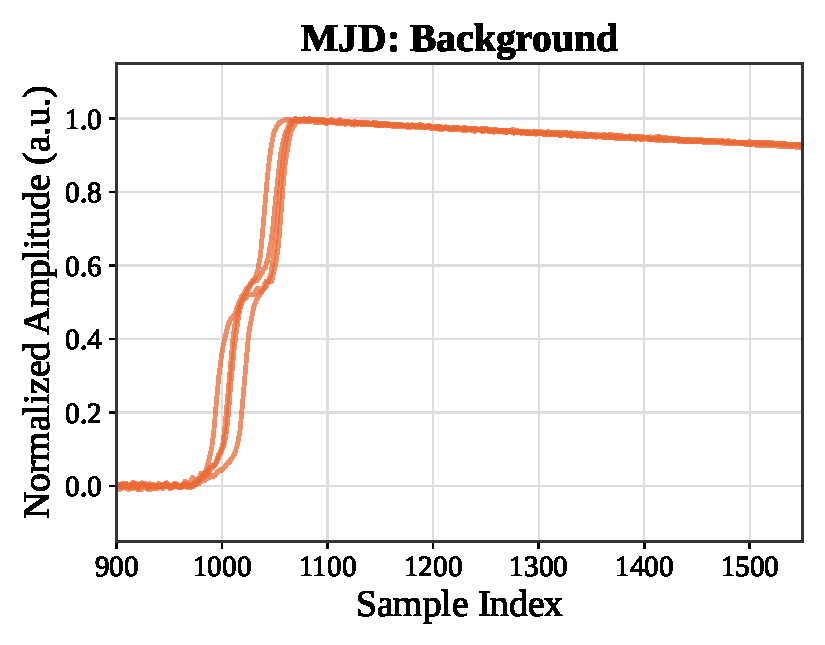
\includegraphics[width=\linewidth,height=3.4cm,keepaspectratio]{dataset_description/Images/mjd_background.pdf}\\[2pt]
        {\small (e) Majorana Demonstrator}
    \end{minipage}
    \hspace{2mm}
    \begin{minipage}[b]{0.23\linewidth}
        \centering
        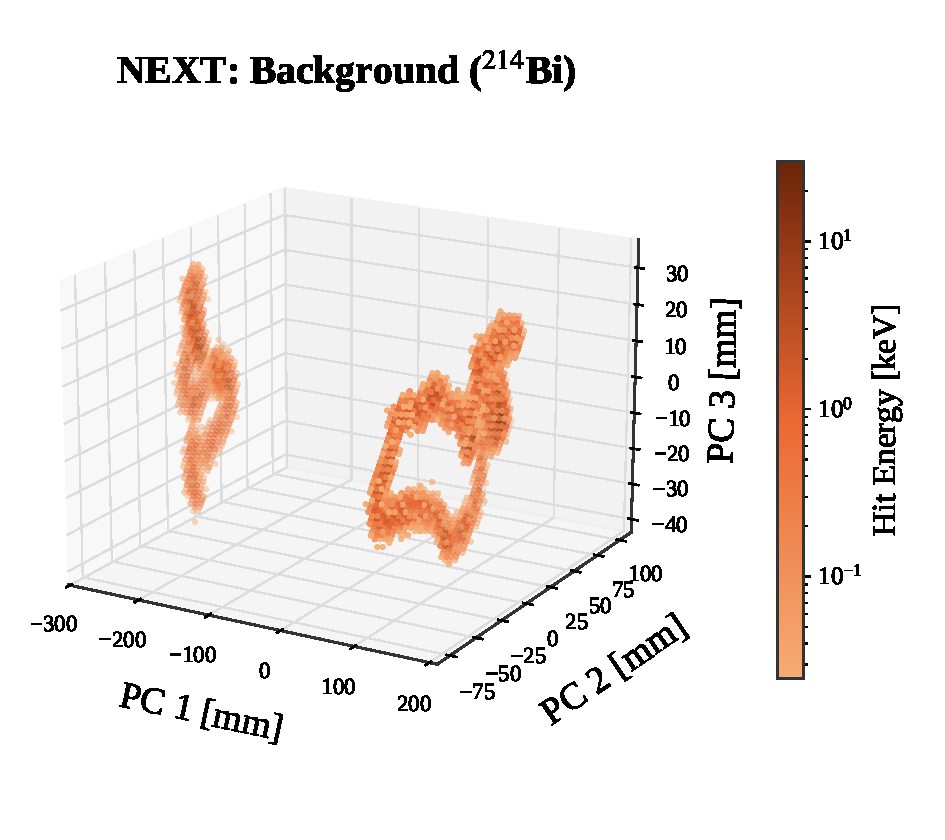
\includegraphics[width=\linewidth,height=3.4cm,keepaspectratio]{dataset_description/Images/next_background.pdf}\\[2pt]
        {\small (f) NEXT}
    \end{minipage}
    \hspace{2mm}
    \begin{minipage}[b]{0.23\linewidth}
        \centering
        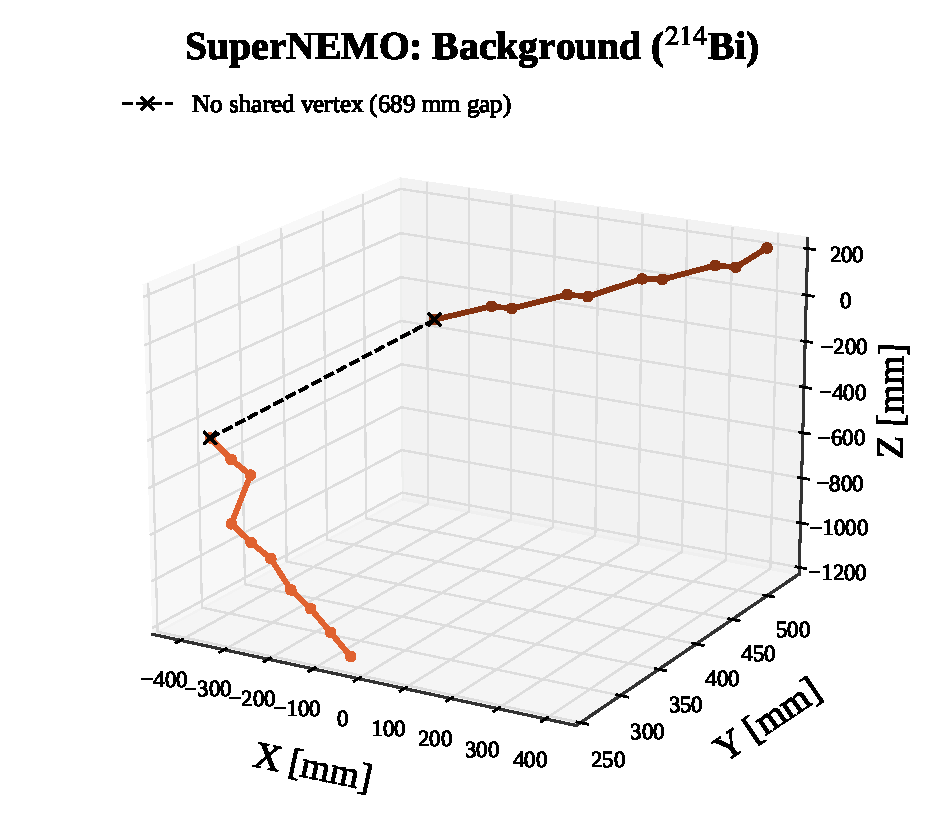
\includegraphics[width=\linewidth,height=3.4cm,keepaspectratio]{dataset_description/Images/supernemo_background.pdf}\\[2pt]
        {\small (g) SuperNEMO}
    \end{minipage}
    \hspace{2mm}
    \begin{minipage}[b]{0.23\linewidth}
        \centering
        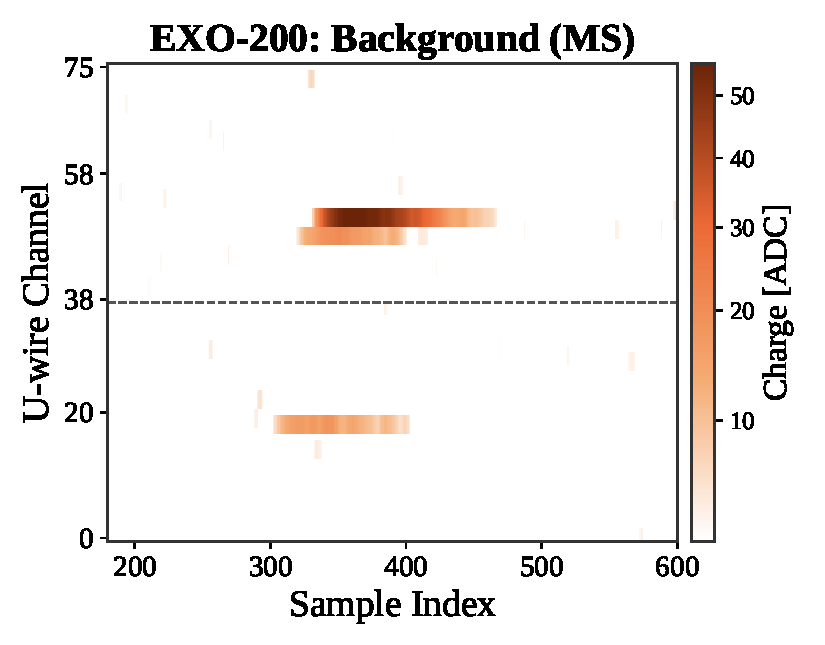
\includegraphics[width=\linewidth,height=3.4cm,keepaspectratio]{dataset_description/Images/exo_background.pdf}\\[2pt]
        {\small (h) EXO-200}
    \end{minipage}
    \caption{Signal (top) versus background (bottom) examples for the four
    experiments, each in its native data modality and each illustrating the
    feature that separates the two classes. Majorana Demonstrator: a
    PSD-accepted waveform with a single sharp rise (a) versus a PSD-rejected
    multi-site waveform whose rise shows a visible second step (e). NEXT: a
    NLDBD 3D hit cloud forming one continuous track (b) versus a
    $^{214}$Bi event whose hits split into two spatially disconnected
    clusters (f). SuperNEMO: a NLDBD candidate whose two
    reconstructed electron tracks meet at a common vertex (c) versus a
    $^{214}$Bi candidate whose tracks share no vertex, with a 689\,mm gap
    between their closest points (g). EXO-200: U-wire (charge-collection)
    channel versus time, where a single-site event produces one collection
    pulse (d) and a multi-site event produces several separated pulses
    across both TPC halves (h); the dashed line separates the two halves.
    Signal is shown in blue and background in orange throughout.}
    \label{fig:signal_background}
\end{figure}
